% CHAPTER - Problem and Challenges ---------------
\chapter{Abordagem proposta}

    Tendo em vista recorrer ao conhecimento obtido na análise do estado da arte, em especial pela identificação das técnicas mais promissoras e as suas respetivas limitações e falhas, realiza-se nesta secção a proposta de uma solução tal como a sua margem de aplicação.

    Pelas suas vantagens relativas à praticamente completa automatização do processo sem necessidade de \textit{inputs} e pré-processamentos elevados por parte do utilizador, nem necessidade de impactos significativos na \textit{performance} de \textit{runtime} da aplicação por necessidade de extração de \textit{logs}, optou-se pelo seguimento de uma abordagem orientada ao código fonte estática.
    
    Esta abordagem terá como base a utilização de um \textit{System Dependence Graph} sobre o qual serão aplicados algoritmos de \textit{clustering} recorrendo a uma análise de critérios de acoplamento identificados pela literatura, nomeadamente os destilados por \cite{gysel16_service_cutter}.
    
    Após a identificação de propostas de micro-serviços será realizada a extração recorrendo a \textit{code slicing}. A aplicação de \textit{code slicing} relativamente a um grafo como o \textit{System Dependence Graph} o qual representa uma granularidade fina do programa, ao nível de \textit{statements}, permitirá uma maior liberdade e melhor manipulação no \textit{refactoring} para micro-serviços mais concisos. Um dos principais objetivos com esta abordagem será trazer o máximo de valor ao desenvolver com um \textit{input} e pré-processamento baixo da sua parte.
    
\section{Âmbito de ação}

    Dada a elevada complexidade em criar uma solução generalizada para múltiplas linguagens e \textit{frameworks} o âmbito de ação para a solução teve de ser reduzido a algo mais específico e manejável.
    
    Começando pela escolha de linguagem, destacam-se como linguagens \textit{web} em especial \textit{PHP, Javascript, Java, C\# e Python}. Apesar da grande utilização de \textit{PHP} dada a tão popular \textit{stack LAMP} e a sua utilização em sistemas de gestão de conteúdo como o \textit{Wordpress}, esta é uma linguagem que não teve particular adaptação no mundo dos micro-serviços por estar em decadência de popularidade. O uso de \textit{PHP} só faria sentido se fosse também realizado o \textit{transpiling} para uma linguagem com melhor adaptação ao mundo dos micro-serviços. O \textit{Javascript} e em particular \textit{frameworks} como o \textit{node} ganharam uma elevada popularidade nos últimos anos sendo utilizados massivamente quer em projetos de pequena dimensão, como em projetos de grande escala que necessitam de ser facilmente escaláveis. Embora esta combinação de \textit{Javascript} e \textit{node} seja bastante popular e fizesse sentido no contexto de utilização de micro-serviços, muitas das aplicações começaram já a ser desenvolvidas durante o ganho de popularidade dos micro-serviços. Das restantes linguagens identificadas destaca-se o \textit{Java} por ser uma linguagem muito utilizada na indústria em especial para sistemas que necessitam que a linguagem lhes permita o desenvolvimento de aplicações robustas. O facto de se ter mantido ao longo dos anos como uma escolha sólida e popular para aplicações \textit{web} e existirem uma elevada quantidade de aplicações monolíticas é também um ponto a seu favor.
    
    A escolha da \textit{framework} a abordar é também importante, dado a diversidade de métodos de desenvolvimento criadas pelas diversas arquiteturas inerentes das \textit{frameworks} e a possibilidade da informação por ela utilizada potenciar o trabalho de identificação e extração de micro-serviços por transmitir contexto extra sobre o código. Num estudo realizado pela \cite{java_frameworks} envolvendo 2060 participantes da área do desenvolvimento de \textit{software}, demonstraram tal como em anos anteriores a alta utilização de \textit{Spring} relativamente a outras \textit{frameworks}, Figura \ref{fig:java_frameworks}. 
    
    
   	\begin{figure}[h!]
     	\begin{center}
     		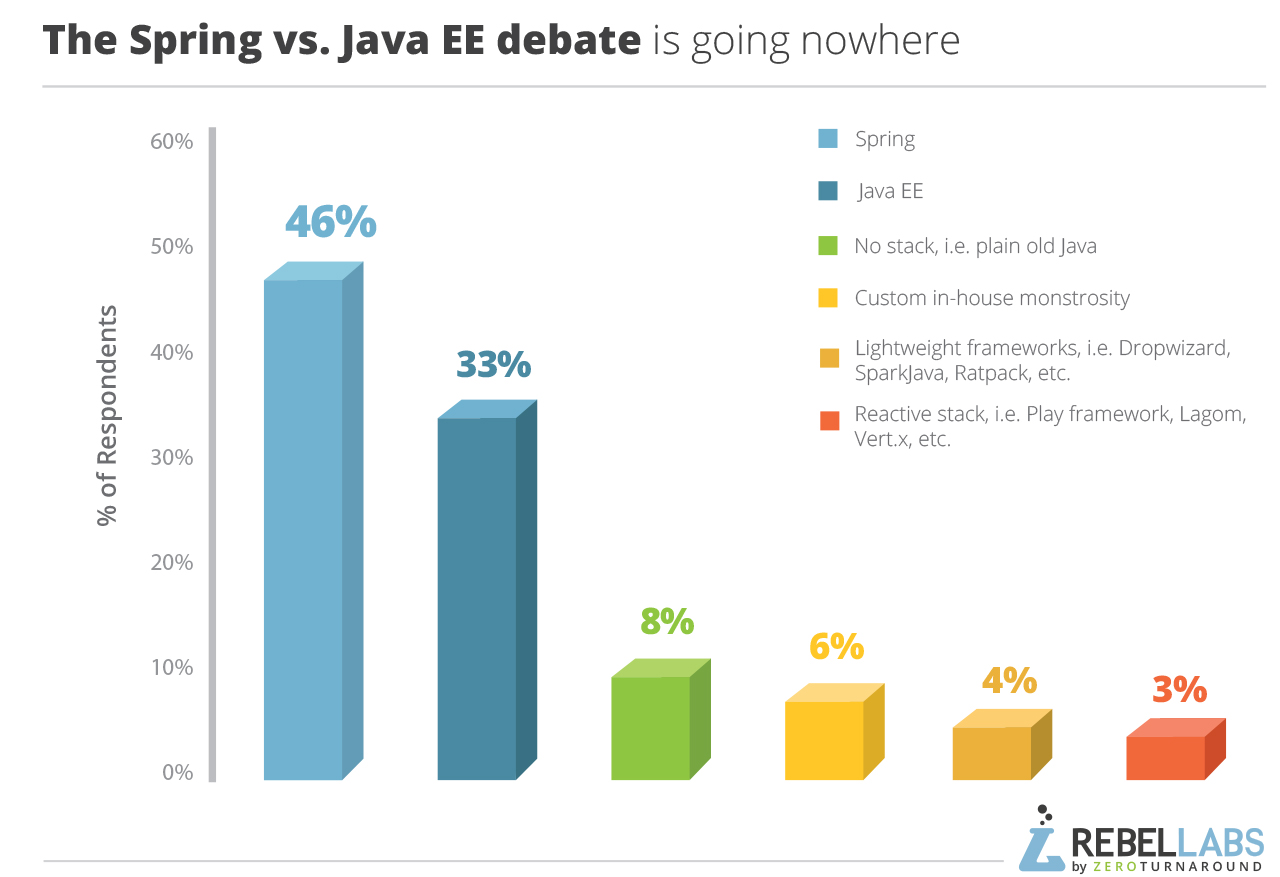
\includegraphics[width=12cm]{img/java_frameworks.jpg}
     	\end{center}
     	\caption{Resultados de um \textit{survey} sobre o uso de \textit{frameworks} Java}
     	\floatfoot{Source: \cite{java_frameworks}}
     	\label{fig:java_frameworks}
 	\end{figure} 
    
    A abordagem escolhida será então aplicada a aplicações \textit{web} desenvolvidas em \textit{Java} recorrendo à \textit{framework Spring}.
    
\section{Validação}

    Um fator fulcral para avaliar a utilidade do trabalho e os seus contributos para com o estado da arte, trata-se da realização da validação do mesmo. Uma das dificuldades neste processo de validação passa pela falta de um consenso sobre o que são ao certo micro-serviços bem definidos, bem aplicados e de qualidade. Começando pelo seu tamanho a nível de linhas de código, existe a regra geral de que devem ser mantidos pequenos, mas o quão pequeno não é consensual, variando de indicações de poucas dezenas de linhas de código, podendo mesmo disponibilizar apenas uma função, a milhares de linhas de código.
    
    Fundamentalmente, um dos principais objetivos dos micro-serviços passa pela facilidade em introduzir e realizar mudanças. Sendo este processo difícil de avaliar recorrendo apenas a métricas, opta-se pela realização de um estudo empírico e qualitativo de várias aplicações no seu estado monolítico e pós-migração. Recorrer-se-á a desenvolvedores de \textit{software} que realizarão uma avaliação qualitativa sobre aspetos como facilidade de introdução de mudanças, adequação dos serviços ao domínio do problema, etc. Esta validação será realizada sobre um repositório de aplicações compostas por ambas as vertentes, aplicação monolítica e micro-serviços.
    
    
\section{Calendarização}

    Apresenta-se de seguida a calendarização expectável com algumas das principais etapas à realização deste trabalho:
    
    \textbf{Etapa 1 - Criação do \textit{SDG} inter-classe}. Para a obtenção do \textit{SDG} recorrer-se-á a uma aplicação que fornece o \textit{SDG} a um nível intra-classe, sendo necessário a adição de funcionalidade para construção do \textit{SDG} inter-classe (ex.: seguimento de execução de métodos correspondentes a outra classe).
    
    \textbf{Etapa 2 - Análise critérios acoplamento e algoritmos de \textit{clustering}} - Nesta fase realizar-se-á a análise para procurar identificar os métodos mais promissores à solução do problema, quer a nível de acoplamento, que servirão para a atribuição de pesos entre ligações, quer a nível de algoritmos de \textit{clustering} que utilizarão os pesos atribuídos para identificar micro-serviços.
    
     \textbf{Etapa 3 - Aplicação dos algoritmos de \textit{clustering}} - Nesta fase será feita a aplicação dos algoritmos de \textit{clustering} dados como promissores na fase anterior sobre o \textit{SDG}.
   
     \textbf{Etapa 4 - Extração dos micro-serviços} - Realiza-se aqui a extração dos micro-serviços tendo em conta os \textit{clusters} de código obtidos, ou seja, o grafo de dependências processado será fragmentado em vários serviços recorrendo a técnicas de \textit{code slicing}.
     
     \textbf{Etapa 5 - Validação e testes} - Após a respetiva implementação realizar-se-á a validação empírica de um conjunto de aplicações.
     
     
     
     \textbf{Etapa 6 - Documentação e escrita da dissertação}.
    
    
    A alocação temporal das tarefas referidas pode ser observada na Figura \ref{fig:gantt}.
    
     
\begin{figure}[htb]
\centering{
\resizebox{\textwidth}{!}{\begin{ganttchart}[y unit title=0.4cm,
    y unit chart=0.5cm,
    vgrid,hgrid,
    title height=1,
    bar/.style={draw,fill=grey},
    bar incomplete/.append style={fill=yellow!50},
    bar height=0.7]{1}{35}
     \gantttitle{Fev}{3}
     \gantttitle{Mar}{4}
     \gantttitle{Abr}{4}
     \gantttitle{Mai}{4}
     \gantttitle{Jun}{4}
     \gantttitle{Jul}{4}
     \gantttitle{Ago}{4}
     \gantttitle{Set}{4}
     \gantttitle{Out}{4}
     % \gantttitlelist{20,...,31}{1}
     % \gantttitlelist{1,...,12}{1} \\
     \\
     \ganttbar{Etapa 1}{1}{4} \\
     \ganttbar{Etapa 2}{5}{7} \\
     % rever estes 2 pontos, sobrepõem-se um pouco, talvez extração e posteriormente migração
     
     % justificar bem as tarefas
     % sugestão: aplicar métodos de clustering
     \ganttbar{Etapa 3}{8}{17} \\
     \ganttbar{Etapa 4}{18}{24} \\
     \ganttbar{Etapa 5}{25}{30} \\
     \ganttbar{Etapa 6}{6}{34} 
\end{ganttchart}}}
\caption{Alocação de tarefas}\label{fig:gantt}
\end{figure}
    
  
% limitações: precisa de seguir um ORM